\documentclass[12pt]{book}
\usepackage[top=1in, bottom=1in, left=1.2in, right=1in, a4paper]{geometry}

 \ifx\pdftexversion\undefined
 \usepackage[dvips]{graphicx}
 \else
 
 \usepackage[pdftex]{graphicx}
 \DeclareGraphicsRule{*}{mps}{*}{}
 \fi
%\usepackage{tabularx,colortbl}
\usepackage{url}
\usepackage{chapterbib}
\usepackage{hyperref}
%\usepackage{tikz}
%\usepackage{pgfplots}
%\usepgfplotslibrary{groupplots} 
%\usepackage{pgf, pgfarrows, pgfnodes}
\usepackage{lscape}
\usepackage{longtable}
\usepackage{float}
\usepackage{url}
\usepackage{multicol}
\usepackage{color}
\usepackage{multirow}
\usepackage{listings}
\usepackage{subfigure}
\usepackage{tabularx,ragged2e,booktabs,caption}

%\usepackage[none]{hyphenat}
\renewcommand{\bibname}{References}
\newcommand{\shellcmd}[1]{\\\indent\texttt{\footnotesize #1}\\}

\setcounter{secnumdepth}{4}
\setcounter{tocdepth}{4}

\begin{document}

\begin{titlepage}
 \begin{center}
\Huge
\textbf{IITB Summer Internship 2014} \\
\vfill

\includegraphics[width=3cm]{IITB_logo.png}
\vfill
\Huge
\textbf{Project Report}\\
\vfill
\textbf{Load Testing and Benchmarking for BigData}\\
\vfill
\LARGE
\underline{\textbf{Principal Investigator}} \\
Prof. D.B. Phatak\\
\vfill
\LARGE
\underline{\textbf{Project In-Charge}} \\
Mr. Nagesh Karmali\\
\vfill
\Large

\begin{tabular}{l|l}
\textbf{Project Mentors} & \textbf{Project Team Members} \\
 & Jayam Modi \\
Mr. Pqr & Sunil Raiyani \\ 
 & Aayush Agrawal\\
\end{tabular}
\vfill

\includegraphics[width=2.5cm]{svnit.jpg} \hfill

\includegraphics[width=2.5cm]{manit.jpg} \hfill
\vfill
\today
\end{center}
\end{titlepage}

 \pagebreak \textcolor{white}{text} \pagebreak
%\setcounter{page}{1}
%\pagenumbering{roman}
\thispagestyle{empty}

\begin{center}
\thispagestyle{empty}
\LARGE
\textbf{Summer Internship 2014 \\ Project Approval Certificate} \\
\vskip12pt
\Large
\textbf{Department of Computer Science and Engineering} \\
\vskip5pt
\textbf{Indian Institute of Technology Bombay} \\
\end{center}
\vfill
\normalsize
The project entitled ``Load Testing and Benchmarking for Bigdata'' submitted by Jayam Modi, Sunil Raiyani, Aayush Agrawal,  is approved 
for Summer Internship 2014 programme from 10th May 2014 to 6th July 2014, at Department of Computer Science and Engineering, IIT Bombay.

\vfill

\begin{multicols}{2}
\underline{\hspace{5cm}} \\
\indent Prof. Deepak B. Phatak \\
\indent Dept of CSE, IITB \\
\indent Principal Investigator \\

\begin{flushright}
\underline{\hspace{5cm}} \\
 Mr. Nagesh Karmali \\
\indent Dept of CSE, IITB \\
\indent Project In-charge \\
\end{flushright}
\end{multicols}

\vfill

\begin{center}
\underline{\hspace{5cm}} \\
 Mr. Pqr \\
 Dept of CSE, IITB \\
 External Examiner \\
 \end{center}
 
 
 \vfill
 Place: IIT Bombay, Mumbai \\
\indent Date: \today

 \pagebreak \thispagestyle{empty} \textcolor{white}{text} \pagebreak
 
\LARGE
\thispagestyle{empty}

\begin{center}
\textbf{Declaration}
\end{center}
\normalsize
I declare that this written submission represents my ideas in my own words and where 
others' ideas or words have been included, I have adequately cited and referenced the original 
sources.  I also declare that I have adhered to all principles of academic honesty and integrity 
and   have   not   misrepresented   or   fabricated   or   falsified   any   idea/data/fact/source   in   my 
submission.  I understand that any violation of the above will be cause for disciplinary action 
by the Institute and can also evoke  penal action from the sources which have thus not been 
properly cited or from whom proper permission has not been taken when needed.

\vfill
\begin{flushright}

\underline{\hspace{5cm}} \\
Jayam Modi \\
Sardar Vallabhbhai National Institute of Technology, Surat \\

\vfill

\underline{\hspace{5cm}} \\
Sunil Raiyani  \\ 
Sardar Vallabhbhai National Institute of Technology, Surat \\

\vfill

\underline{\hspace{5cm}} \\
Aayush Agrawal \\
Maulana Azad National Institute of Technology, Bhopal \\

\vfill
\end{flushright}

\textbf{Date:} \underline{\hspace{5cm}}

\chapter*{Abstract}
\setcounter{page}{1}
\pagenumbering{roman}
Write your abstract here

\listoffigures
\listoftables
\tableofcontents

\pagebreak
\cleardoublepage

\setcounter{page}{1}
\pagenumbering{arabic}

\chapter{Introduction to BigData and Benchmarking}
\section{Introduction}
The project is about Load Testing and Benchmarking for BigData. A distributed file system setup is generated using a cluster consisting of 
multiple nodes. Complex data sets are generated and the data is processed using distributed processing tools to produce meaningful results.
\\\noindent
\section{Load Testing}
It means to test the system by steadily increasing the load on the system till it reaches its threshold limit. In the current case, 
the size of the dataset is increased until it becomes impossible for the cluster to process the data. It helps to identify the maximum 
operating capacity of the system and the bottlenecks if any. The components causing degradation are easily identified using load testing.
\\\noindent
\section{Benchmarking}
It refers to the process of comparing the performance metrics of own systems with the industry standards. It is performed using 
a specific indicator which becomes a performance metric for comparision. Its aim is to help evolve systems in those areas where they are
weak in performance. Benchmarking software can be used to organize huge and complex information.
\\\noindent
\section{BigData}
It is a term that covers data sets so large and complex that it becomes impossible to process them using on-hand database management tools and 
traditional data processing applications. Relational database management systems fail to perform when it comes to BigData. It largely involves
unstructured data which is not possible to capture and process using DBMS or RDBMS. The only possible way to process BigData is using 
parallel and distributed database systems. BigData sets are so large that their size is measured in terms of exabytes (2*10$^{18}$ bytes).
It is currently impossible for any single system to store and process such a huge amount of data on its own.
\section{Hadoop}
Apache Hadoop is an open-source framework that can be used for storing  and processing large and complex data sets on clusters made up of
commodity hardware systems. It provides a Distributed file system named HDFS which is a platform to store huge amounts of data  divided into 
blocks across multiple hosts. It also provides the MapReduce Engine which performs the processing of BigData.
\\\noindent


%%%%%%%%%%%%%%%%%%%%%%%%%%%%%%%%%%%%%%%%%%%%%%%%%%%%%%%%%%%%%%%%%%%%%%%%%%%%%%%%%%%%%%%%%%%%%%%%%%%%%%%%%%%%%%%%%%%%%%%%%%%%%%%%%%%%%%%%%%%%%%
%%%%%%%%%%%%%%%%%%%%%%%%%%%%%%%%%%%%%%%%%%%%%%%%%%%%%%%%%%%%  Apache Hadoop  %%%%%%%%%%%%%%%%%%%%%%%%%%%%%%%%%%%%%%%%%%%%%%%%%%%%%%%%%%%%%%%%%
%%%%%%%%%%%%%%%%%%%%%%%%%%%%%%%%%%%%%%%%%%%%%%%%%%%%%%%%%%%%%%%%%%%%%%%%%%%%%%%%%%%%%%%%%%%%%%%%%%%%%%%%%%%%%%%%%%%%%%%%%%%%%%%%%%%%%%%%%%%%%%

\chapter{Apache Hadoop}
\section{Introduction}
The Apache Hadoop software library is a framework that allows for the distributed processing of large data sets across clusters of computers using simple programming models. It is designed to scale up from single servers to thousands of machines, each offering local computation and storage.
The project includes these modules: 
\begin{itemize}
 \item Hadoop Common
 \item Hadoop Distributed File System
 \item Hadoop Yarn
 \item Hadoop MapReduce
\end{itemize}
\subsection{Hadoop Common}
Hadoop Common is the set of common utilities that support other Hadoop modules.
In this section :
\begin{itemize}
 \item Using File System(FS) shell commands: The File System (FS) shell includes various shell-like commands that directly interact with the Hadoop Distributed File System (HDFS)\\
 Various commands are:
 \begin{enumerate}
   \item cat: Copies source paths to stdout.\\
   \hspace{40mm} hdfs dfs -cat file:///file3 /user/hadoop/file4
   \item chmod: Change the permissions of files. With -R, make the change recursively through the directory structure. The user must be the owner of the file, or else a super-user.
   \item chown: Change the owner of files. With -R, make the change recursively through the directory structure. The user must be a super-user.
   \item copyFromLocal: Copy single src, or multiple srcs from local file system to the destination file system.\\
   Usage: hdfs dfs -copyFromLocal $<$localsrc$>$ URI
   \item copyToLocal:Copy files to the local file system.\\
   Usage: hdfs dfs -copyToLocal [-ignorecrc] [-crc] URI $<$localdst$>$
   \end{enumerate}

 \item Hadoop Commands References: All hadoop commands are invoked by the bin/hadoop script. Running the hadoop script without any arguments prints the description for all commands.
   \begin{enumerate}
   \item fsck: Runs a HDFS filesystem checking utility.It is used to find out which files and blocks are corrupt.
   \item jar: Runs a jar file. Users can bundle their Map Reduce code in a jar file and execute it using this command.\\
   Usage: hadoop jar $<$jar$>$ [mainClass] args...
   \item version: Prints the current version.
   \item dfsadmin: Runs a HDFS dfsadmin client.\\
   Usage: hadoop dfsadmin -report: Reports basic filesystem information and statistics.
  
  
   \end{enumerate}
\end{itemize}


\subsection{Hadoop Distributed File System}
HDFS is a distributed file system that provides high-throughput access to data.
It provides a limited interface for managing the file system to allow it to scale and provide high throughput. 
HDFS creates multiple replicas of each data block and distributes them on computers throughout a cluster to enable reliable and rapid access.\cite{Features}\\
\begin{figure}[hb]
 \centering
 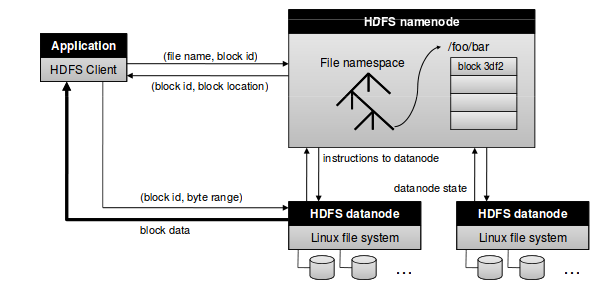
\includegraphics[width=15cm]{./hadoop_archi.png}
 \caption{Hadoop Architecture } 
\end{figure}
\begin{enumerate}
\item Namenode and Datanode:
The distributed file system adopts a master slave architecture in which
the namenode maintains the file namespace (metadata, directory structure, file to block
mapping, location of blocks, and access permissions) and the datanodes manage the actual data
blocks.
\item Relationship between Namenode and Datanode:
Data nodes continuously loop, asking the name node for instructions by sending heartbeat messages. 
A name node can't connect directly to a data node; it simply returns values from functions invoked by a data node.
Each data node maintains an open server socket so that client code or other data nodes can read or write data.

\item Data Replication:
HDFS replicates file blocks for fault tolerance. An application can specify the number of replicas of a file at the time it is created, and this number can be changed any time after that. 
The name node makes all decisions concerning block replication.The namenode attempts to optimize communications between data nodes. The namenode identifies the location of data nodes by their rack IDs. 

\item Data Organization:
Hadoop primary goal is to store large datafiles.The default size of typical datablock is 64MB.It can be configured by changing the core-site.xml file.
HDFS tries to place each block on separate data nodes.

\item Data Block Rebalancing:
HDFS data blocks might not always be placed uniformly across data nodes,
meaning that the used space for one or more data nodes can be underutilized.
It provides hadoop balance command for manually rebalancing task.

\item Snapshots:
HDFS was originally planned to support snapshots that can be used to roll back a corrupted HDFS instance to a previous state.
\end{enumerate}
\subsection{Hadoop Yarn}
The fundamental idea of YARN is to split up the two major responsibilities of the JobTracker 
i.e.resource management and job scheduling/monitoring, into separate daemons:a global ResourceManager and per-application ApplicationMaster (AM)\\
The ResourceManager and per-node slave, the NodeManager (NM), form the new, and generic, system for managing applications in a distributed manner.\\ 
The ResourceManager is the ultimate authority that arbitrates resources among all the applications in the system.\\
The Hadoop Yarn architecture can be seen here \ref{fig:fig1_yarn}
\begin{figure}[ht]
 \centering
 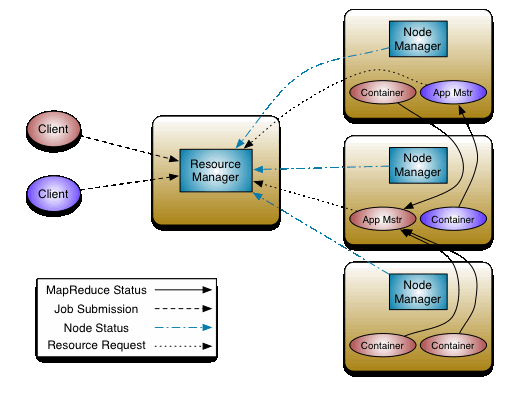
\includegraphics[height=10cm,width=15cm]{./yarn_archi.png}
 \caption{Yarn Architecture\label{fig:fig1_yarn}}
\end{figure}
\subsection{Hadoop MapReduce}
A MapReduce job usually splits the input data-set into independent chunks which are processed by the map tasks in a completely parallel manner.
The framework takes care of scheduling tasks, monitoring them and re-executes the failed tasks.\cite{mapreduce} 
The MapReduce framework consists of a single master JobTracker and one slave TaskTracker per cluster-node. The master is responsible for scheduling the jobs' component tasks on the slaves, monitoring them and re-executing the failed tasks. 
The slaves execute the tasks as directed by the master.

The MapReduce framework operates exclusively on $<$key, value$>$ pairs, that is, the framework views the input to the
job as a set of $<$key, value$>$ pairs and produces a set of $<$key, value$>$ pairs as the output of the job, 
mainly of different types.\\
\textbf{MapReduce-Interfaces}
\begin{itemize}
 \item Mapper: Maps are the individual tasks that transform input records into \\
 intermediate records. The transformed intermediate records do not need to be of the same type as the input records. 
 A given input pair may map to zero or many output pairs.
 \item Reducer: It reduces a set of intermediate values which share a key to a smaller set of values
 \item Partitioner: It controls the partitioning of the keys of the intermediate \\
 map-outputs. The key (or a subset of the key) is used to derive the partition, typically by a hash function.
 \item Combiner: They are an optimization in MapReduce that allow for local\cite{PNC} \\
 aggregation.Combiners works  as mini-reducers that take place on the output of the mappers.\ref{fig1mapred}
\end{itemize}
\begin{figure}[ht]
 \centering
 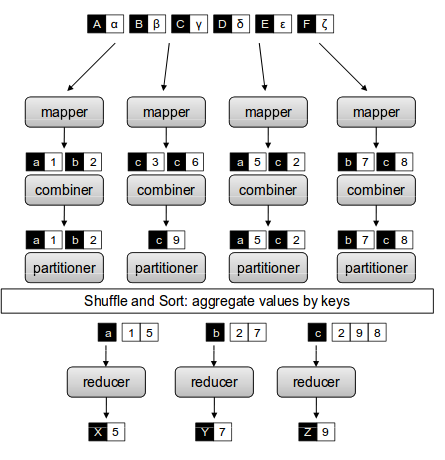
\includegraphics[height=10cm,width=10cm]{./mapper.png} 
 \caption{Complete View of MapReduce\label{fig1mapred}}
\end{figure}

\section{Installation}
The main goal of this tutorial is to get a simple Hadoop installation up and running so that we could learn more internals about it.
This tutorial has been tested on \cite{single}
\begin{enumerate}
 \item Ubuntu Linux 14.04 LTS
 \item Hadoop 2.2 released on October 2013
\end{enumerate}
\subsection{Single Node Cluster}
\begin{itemize}
 \item Prerequisites
\begin{enumerate}
 \item Hadoop Client/User
       \shellcmd{sudo addgroup hadoop  \\\indent 
                sudo adduser –ingroup hadoop hduser \#\# Name assigned to the client groups\\\indent 
                sudo adduser hduser sudo\\\indent
                }
 \item Java jdk(6 or higher)
       \shellcmd{sudo apt-get install openjdk-7-jdk  \\\indent 
                 cd /usr/lib/jvm \\\indent 
                 ln -s java-7-openjdk-amd64 jdk\\\indent
                 }
  \item SSH
        \shellcmd{sudo apt-get install openssh-server  \\\indent 
                  ssh-keygen -t rsa -P ”” \\\indent 
                  ssh localhost\\\indent 
                 }
\end{enumerate}
\item Installing Hadoop-Download and Environment:
\begin{enumerate}
 \item Download 
       \shellcmd{wget http://apache.mirrors.lucidnetworks.net/hadoop/common/stable/hadoop-
2.2.0.tar.gz \\\indent 
                sudo tar vxzf hadoop-2.2.0.tar.gz -C /usr/local \\\indent 
                cd /usr/local\\\indent 
               sudo mv hadoop-2.2.0 hadoop\\\indent 
                sudo chown -R hduser:hadoop hadoop\\\indent}

 \item Enviornment Set-up :Add following to .bashrc file
        \shellcmd{export JAVA\_HOME =/usr/lib/jvm/jdk/ \\\indent 
                  export HADOOP\_INSTALL=/usr/local/hadoop  \\\indent 
                  export PATH=$PATH:$HADOOP\_INSTALL/bin\\\indent 
                  sudo mv hadoop-2.2.0 hadoop\\\indent 
                  sudo chown -R hduser:hadoop hadoop\\\indent}
  
       
\end{enumerate}
\item Installing Hadoop-Configuration and Launching: 
\begin{enumerate}
 \item User based configuration: change the extension of configuration file 
       \shellcmd{/usr/local/hadoop/etc/hadoop/core-site.xml \\\indent 
                /usr/local/hadoop/etc/hadoop/hdfs-site.xml \\\indent 
                /usr/local/hadoop/etc/hadoop/yarn-site.xml\\\indent 
                /usr/local/hadoop/etc/hadoop/mapred-site.xml\\\indent}

 \item Launch
        \shellcmd{mkdir -p mydata/hdfs/namenode\\\indent 
                  mkdir -p mydata/hdfs/datanode  \\\indent 
                  hdfs namenode -format\\\indent 
                  start-dfs.sh\\\indent 
                  start-yarn.sh\\\indent                }
        
\end{enumerate}
\end{itemize}

\subsection{Multi Node Cluster}
\begin{itemize}

\item Prerequisites 
Install the single node cluster on every node and try to run some task on these nodes.\cite{multi}
\item Network Settings 
To run a nulti-node cluster ensure that master and slave are on the same network.Identify the ip address of each node.
Now make entries in the /etc/hosts file as follows:\\
10.129.46.111 master\\
10.129.46.113 slave\\\indent

\item SSH Access 
Add the public key of master to all the slaves using the command:
\shellcmd{hduser@master:~\$ ssh-copy-id -i \$HOME/.ssh/id\_rsa.pub hduser@slave}\\
Now ssh to master and slaves ensuring the passwordless access.
\shellcmd{ssh master}
\shellcmd{ssh slave}

\item Configuration files 
Add the following lines between $<$configuration$>$ ans $<$/configuration$>$ tags to the file in \$HADOOP\_HOME/etc/hadoop
for both master and slave.
\begin{enumerate}
\item Core-xite.xml
       \shellcmd{$<$property $>$\\\indent 
                $<$name$>$fs.defaultFS $<$/name$>$ \\\indent 
                $<$value$>$hdfs://master:9000 $<$/value$>$\\\indent 
                $<$/property$>$\\\indent}

 \item yarn-site.xml
       \shellcmd{$<$property $>$\\\indent 
                $<$name$>$yarn.nodemanager.aux-services$<$/name$>$ \\\indent 
                $<$value$>$mapreduce\_shuffle $<$/value$>$\\\indent 
                $<$/property$>$\\\indent 
                $<$property $>$\\\indent 
                $<$name$>$yarn.nodemanager.aux-services.mapreduce\_shuffle.class $<$/name$>$ \\\indent 
                $<$value$>$org.apache.hadoop.mapred.ShuffleHandler $<$/value$>$\\\indent 
                $<$/property$>$\\\indent}
  \item mapred-site.xml
       \shellcmd{$<$property $>$\\\indent 
                $<$name$>$mapreduce.framework.name$<$/name$>$ \\\indent 
                $<$value$>$yarn$<$/value$>$\\\indent 
                $<$/property$>$\\\indent}
  \item hdfs-site.xml
       \shellcmd{$<$property $>$\\\indent 
                $<$name$>$dfs.replication$<$/name$>$ \\\indent 
                $<$value$>$3$<$/value$>$\\\indent 
                $<$/property$>$\\\indent 
                $<$property $>$\\\indent 
                $<$name$>$dfs.namenode.name.dir$<$/name$>$ \\\indent 
                $<$value$>$file:/home/hduser/mydata/hdfs/namenode$<$/value$>$\\\indent 
                $<$/property$>$\\\indent 
                $<$property $>$\\\indent 
                $<$name$>$dfs.namenode.data.dir$<$/name$>$ \\\indent 
                $<$value$>$file:/home/hduser/mydata/hdfs/datanode$<$/value$>$\\\indent 
                $<$/property$>$\\\indent}
\end{enumerate}
Now add all the slaves name to the \$HADOOP\_HOME/etc/slaves file
\shellcmd{nano \$HADOOP\_HOME/etc/slaves}

\item Launching 
Run the following script in master node
\shellcmd{hdfs namenode -format\\\indent 
                  start-dfs.sh\\\indent 
                  start-yarn.sh\\\indent}
To test whether all the daemon started or not run the jps command on master and slave.\\
\textbf{On Master}
\shellcmd{hduser@master:/usr.local/hadoop\$: jps}
9412   SecondaryNameNode \\
9834   NameNode\\
1056   jps\\
10898  ResourceManager\\
\textbf{On Slave}
\shellcmd{hduser@slave:/usr.local/hadoop\$: jps}
1876   NodeManager \\
9856   DataNode\\
10561  jps\\

\end{itemize}
 
\section{Network Monitoring Tools}
Network monitoring is the use of a system that constantly monitors a computer network or cluster for slow or failing components and that notifies the network 
master (via graphs).There are many networking tools such as Nagios,Ambari etc.
Here ,we have used the ganglia as a monitoring tool.
\subsection{Ganglia}
Ganglia is a scalable distributed monitoring system for high-performance computing systems such as clusters and Grids.
It leverages widely used technologies such as XML for data representation, XDR for compact, 
portable data transport, and RRDtool for data storage and visualization.
It consists of two daemon:
\begin{itemize}
 \item gmond (Ganglia Monitoring Daemon)
 \item gmetad (Ganglia Meta Daemon)
 \end{itemize}
\textbf{gmond} runs on each node you want to monitor. It monitors changes in the host state,
announce relevant changes, listen to the state of all other ganglia nodes via a unicast or
multicast channel and answers requests for an XML.\\
\textbf{gmetad} runs on the master node and gathers all information from the client nodes.
Ganglia also contains a PHP Web Front-end which displays the gathered information in
the form of graphs via web pages.
\\\noindent
\begin{enumerate}
\item \textbf{Installation on Master Node}
The gmond daemon has to be installed on all nodes while the gmetad daemone must only
be installed on the master node. To install ganglia and its web-frontend on the Master
Node, fire the following commands from the terminal.\cite{ganglia}
\shellcmd{sudo apt-get install ganglia-monitor rrdtool gmetad ganglia-webfrontend}\\\noindent
Now edit the /etc/ganglia/gmetad.conf
\shellcmd{sudo nano /etc/ganglia/gmetad.conf}\\\noindent
Find the line of the following type and modify it as follows:
\shellcmd{data\_source "master" 50 127.0.0.1 ip-address-of-namenode}\\\noindent
Here master is the name of cluster. 50 indicates that logs will be collected after every 50 seconds. 127.0.0.1 is ip address of a namenode.\\
Now edit the file /etc/ganglia/gmond.conf
\shellcmd{sudo nano /etc/ganglia/gmond.conf}\\
Find the following lines and make appropriate changes as indicated:
\shellcmd{cluster \{ \\\indent 
name = "master" \#\# Name assigned to the client groups\\\indent 
owner = "unspecified"\\\indent 
latlong = "unspecified"\\\indent 
url = "unspecified"\\\indent}
\shellcmd{udp\_send\_channel \{ \\\indent 
\#mcast\_join=239.2.11.71\\\indent 
host = 10.105.24.11\\\indent 
port = 8649\\\indent 
ttl = 1\\\indent }
\shellcmd{udp\_recv\_channel \{ \\\indent 
port = 8649}
\shellcmd{tcp\_accept\_channel \{ \\\indent 
port = 8649}
The changes in the above configuration file show that the master node which has IP
address 127.0.0.1 will collect data from all nodes on tcp and udp port 8649.
Now start the services using the following commands:
\shellcmd{sudo /etc/init.d/ganglia-monitor restart}
\shellcmd{sudo /etc/init.d/gmetad restart}

\item \textbf{Installation on Slave Node}
Install the ganglia monitor package for all the slave nodes that we want to monitor.
\shellcmd{sudo apt-get install ganglia-monitor}\\\noindent
Now edit the /etc/ganglia/gmond.conf file as follows:
\shellcmd{sudo nano /etc/ganglia/gmond.conf}\\\noindent
Make the following changes:
\shellcmd{cluster \{ \\\indent 
name = "master" \#\# Name assigned to the client groups\\\indent 
owner = "unspecified"\\\indent 
latlong = "unspecified"\\\indent 
url = "unspecified"\\\indent }
\shellcmd{udp\_send\_channel \{ \\\indent 
\#mcast\_join=239.2.11.71\\\indent 
host = 10.105.24.11\\\indent 
port = 8649\\\indent 
ttl = 1\\\indent}
Now restart ganglia-monitor service.
\shellcmd{sudo /etc/init.d/ganglia-monitor restart}
\item \textbf{Using Ganglia}
Start a web browser and type in the following address :
\textbf{http://ip-address-of-namenode/ganglia}\\
A screen similar to the one shown in the figure \ref{fig:fig2_ganglia} appears:
\begin{figure}[hb]
 \centering
 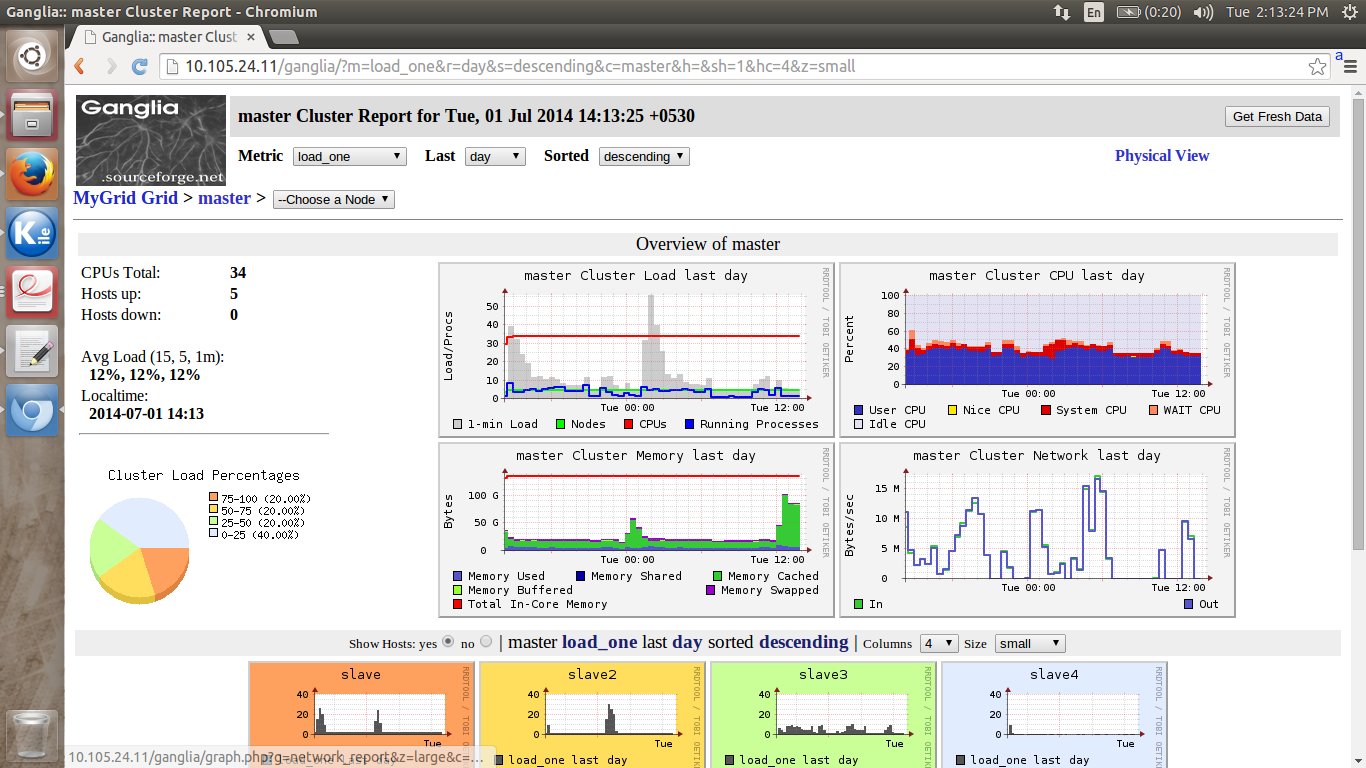
\includegraphics[width=15cm]{./ganglia.png}
 \caption{Ganglia Interface \label{fig:fig2_ganglia}} 
\end{figure}
Select the node that you want to monitor from the list of available nodes.\ref{fig:fig2_ganglia} There are
many graphs for each node which indicate the Memory Usage, CPU utilization, Network
Load and Load Sharing of various nodes.
\end{enumerate}




%%%%%%%%%%%%%%%%%%%%%%%%%%%%%%%%%%%%%%%%%%%%%%%%%%%%%%%%%%%%%%%%%%%%%%%%%%%%%%%%%%%%%%%%%%%%%%%%%%%%%%%%%%%%%%%%%%%%%%%%%%%%%%%%%%%%%%%%%%%%%%
%%%%%%%%%%%%%%%%%%%%%%%%%%%%%%%%%%%%%%%%%%%%%%%%%%%%%%%%%%%%%  Apache Hive  %%%%%%%%%%%%%%%%%%%%%%%%%%%%%%%%%%%%%%%%%%%%%%%%%%%%%%%%%%%%%%%%%%
%%%%%%%%%%%%%%%%%%%%%%%%%%%%%%%%%%%%%%%%%%%%%%%%%%%%%%%%%%%%%%%%%%%%%%%%%%%%%%%%%%%%%%%%%%%%%%%%%%%%%%%%%%%%%%%%%%%%%%%%%%%%%%%%%%%%%%%%%%%%%%

\chapter{Apache Hive}
\section{Overview}
Apache Hive, as reported in \cite{Hive} , is a data warehouse infrastructure built on top of hadoop for providing data analysis and querying features. It was initially 
developed by Facebook but now it is used by many other companies. It supports HiveQL which is a SQL-like declarative language. The queries of
HiveQL are compiled into map-reduce jobs executed on Hadoop. It also supports custom map-reduce scripts which can be inserted into queries.
\section{Data Model}
The Data in hive is organized into Tables, Partitions and Buckets.
\begin{itemize}
 \item \textbf{Tables} - They are similar to tables from RDBMS. Each table is stored on a separate directory on the HDFS. The data is 
 serialized and then stored on the files in the directory.
 \item \textbf{Partitions} - Each table can have multiple partitions which are stored in different subdirectories within the parent directory
 of the table.
 \item \textbf{Buckets} - The data of each partition may be divided into buckets depending on the hash of a column in the table.
 All the buckets are stored in different files within the partition sub-directory.
\end{itemize}
Hive provides primitive(integer, float, string,etc.) as well as custom data types (array and map).
\section{Query Language}
HiveQL supports all types of operations like select, project, aggregate, join, union, etc.
It provides DDL statements to create, modify and delete tables. It also provides DML statements like load and insert to enter data into
tables. HiveQL also supports multi-table insert which allows users to perform multiple queries on a single input data.
\section{Installation}
The following steps must be followed inorder to install hive on a system:
\begin{enumerate}
 \item \textbf{Prerequisites}
 \\\indent Setup Hadoop-2.2.0 using the steps mentioned in the previous chapter.
 \item \textbf{Download Hive}
 \\\indent Download the lastest version of hive from apache-hive's repository.
  \shellcmd{wget http://apache.mirrors.hoobly.com/hive/stable/apache-hive-0.13.0-bin.tar.gz}
 \item \textbf{Extract Hive}
 \\\indent Extract the files to a directory and then move the directory to a proper location.
 \shellcmd{sudo tar -zxvf apache-hive-0.13.0-bin.tar.gz\\\indent
  sudo mv apache-hive-0.13.0-bin /usr/local/hive\\\indent
  sudo chown -R hduser:hadoop hive
 }
 \item \textbf{Setup Environment Variables}
 \\\indent Add the following lines to ~/.bashrc file
 \shellcmd{export HIVE\_PREFIX=/usr/local/hive\\\indent
 export PATH=\$PATH:\$HIVE\_PREFIX/bin
 }Now logout and then login again inorder to set the enviroment variables.
 \item \textbf{Using Hive}
 \\\indent Write \textbf{hive} on the terminal in order to open hive. Once opened, it will look like this:
 \shellcmd{hive>}
 Now, HiveQL statements can be used to analyze and manipulate data.
\end{enumerate}



%%%%%%%%%%%%%%%%%%%%%%%%%%%%%%%%%%%%%%%%%%%%%%%%%%%%%%%%%%%%%%%%%%%%%%%%%%%%%%%%%%%%%%%%%%%%%%%%%%%%%%%%%%%%%%%%%%%%%%%%%%%%%%%%%%%%%%%%%%%%%%
%%%%%%%%%%%%%%%%%%%%%%%%%%%%%%%%%%%%%%%%%%%%%%%%%%%%%%%%%%%%%%  Big-Bench  %%%%%%%%%%%%%%%%%%%%%%%%%%%%%%%%%%%%%%%%%%%%%%%%%%%%%%%%%%%%%%%%%%%
%%%%%%%%%%%%%%%%%%%%%%%%%%%%%%%%%%%%%%%%%%%%%%%%%%%%%%%%%%%%%%%%%%%%%%%%%%%%%%%%%%%%%%%%%%%%%%%%%%%%%%%%%%%%%%%%%%%%%%%%%%%%%%%%%%%%%%%%%%%%%%

\chapter{BigBench}
\section{Overview}
BigBench is an industry standard benchmark for big data analytics \cite{ghazal}. All the major characteristics in the lifecycle of a big data 
system are covered in BigBench which is an end-to-end benchmark. The three V's described by Douglas Laney \cite{doug} are the most important
characteristics of a big data system:
\begin{itemize}
 \item \textbf{Volume} - Large data set sizes.
 \item \textbf{Velocity} - Higher data arrival rates such as clickstreams.
 \item \textbf{Variety} - Different data type such as structured (relational tables) , semi-structured (key-value web-clicks) 
  and unstructured (social media content).
\end{itemize}
\section{Data Model}
BigBench is based on a data model of a fictitious retailer who sells products to customers via physical and online stores.
It has been adapted from the TPC-DS data model for relational databases.
The following diagram \ref{schema} explains the data model:
\begin{figure}[hb]
 \centering
 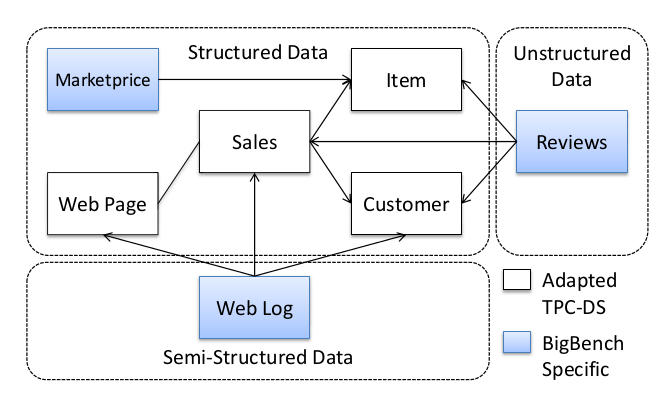
\includegraphics[height=7cm,width=15cm]{Schema.png}
 \caption{Big-Bench Data Model \label{schema}}
\end{figure}
\newpage
\noindent
This model is implemented using a set of 23 tables which contains various columns for storing structured data.
\\\noindent
\\\noindent
The Big-Bench Data model contains the following three types of data -
\begin{itemize}
 \item \textbf{Structured} - The structured part of BigBench is an adaption of the TPC-DS model which also depicts a product retailer model.
 It borrows the store and online sales part from that model and adds a table named ``MarketPrice'' for competitor prices of the retailer.
 \item \textbf{Semi-Structured} - The semi-structured part's content is composed by clicks made by customers and guest users visiting 
 the retailer site. Some of these clicks are for completing a customer order. The design assumes the semi-structured data to be a key-value 
 format similar to Apache web server log format.
 \item \textbf{Un-Structured} - Online Product Reviews serve as a good source of unstructured data.
\end{itemize}
\section{Data Generation}
The Big-Bench data generation scheme is based on a technique called PDGF ( Parallel Data Generation Framework ). PDGF addresses only structured
data by design. But it has been extended to generate semi-structured and unstructured data. PDGF is implemented in Java and is fully
platform independent. The information for data generation is specified in two XML files, schema configuration ( contains data similar
to the relational schema) and generation configuration ( contains additional post processing options ).
\\\noindent
The listing below shows the XML code for defining structured data.
\begin{lstlisting}[frame=single]
<property name = "Item_marketprice" type="double" >
${item }*${avg_competitors_per_item}
</property>
<table name = "Item_marketprice">
<size> ${Item_marketprice} </size>
<field name = " imp_sk " size = " " type ="NUMERIC">
<gen_IdGenerator/>
</field>
[..]
<field name = "imp_competitor" size ="20"
type = " VARCHAR " >
<gen_NullGenerator>
<probability> 0.00025 </probability>
<gen_RandomAString>
<size > 20 </size>
</gen_RandomAString>
</gen_NullGenerator>
</field>
[..]
</table>
\end{lstlisting}
\noindent
To generate a realistic web-log, all the required  coloumns for a web-log entry are specified in a table.
The sizing is computed based on a specific formula. The listing below shows the formatting code for the web-log.
Some of the values are static while others are extracted from the table.
\\\noindent
\begin{lstlisting}[frame=single]
<output name = "CompiledTemplateOutput">
<template> 
<!--
String nl = pdgf.util.Constants.DEFAULT_LINESEPARATOR;
buffer.append("127.0.0.1--["+fields[4]+":"
+fields[5]+"+0200]");
buffer.append("\"GET /page"+fields[7]+".html?");
[..]
buffer.append(" HTTP /1.1\" 200 0 -\" "+fields [1]) ;
buffer.append(" \" \" Mozilla /5.0 \" " + nl) ;
-->
</template>
</output>
\end{lstlisting}
\noindent
The review generator for unstructured data was built as a standalone program which is configured using an XML document that 
specifies the parameters for each review. In order to generate correlated reviews, PDGF is used to generate the XML document
for each review.
The figure \ref{review} shows the process of review generation.
\begin{figure}[hb]
 \centering
 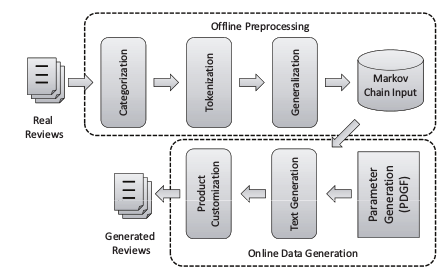
\includegraphics[width=15cm]{review.png}
 \caption{Review Generation Model \label{review}}
\end{figure}
The process can be separated in two phases. An offline phase, that processes real reviews and generates a knowledge 
base for the review generation and an online phase that generates reviews based on the knowledge base.

\section{Workload}
The workload for BigBench considers the initial database population in addition to the queries. This initial phase called
Transformation Ingest (TI) covers all the steps needed to prepare the data before querying.
The main part of the workload however is the set of 30 queries which are executed against the data model. They are designed along one business
dimension and three technical dimensions.
The set of 30 queries is chosen so that the distribution shown in figure \ref{workload} can be obtained.
\begin{figure}[h]
 \centering
 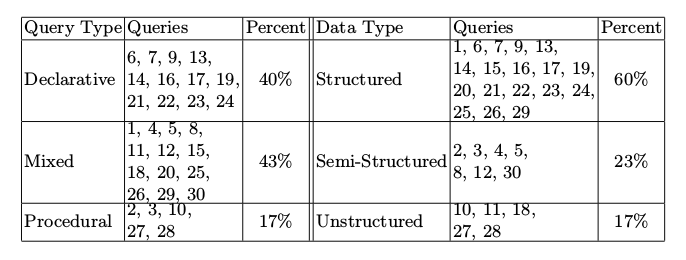
\includegraphics[width=15cm]{workload.png}
 \caption{Workload Distribution \label{workload}}
\end{figure}
The figure clearly indicates that a major proportion of the queries operate on structured data since the data model largely consists of 
structured data.
\section{Benchmark Results}
The set of 30 queries was executed on a 8 node Teradata Aster appliance. Each node was a Dell server with two quad-core Xeon 5500 @ 3.07Ghz and 
hardware RAID 1 with 8 2.5{``} drives. The table \ref{qtime30} shows the times obtained for individual queries.
\captionof{table}{Query Run-Time}
\begin{center}
\begin{tabular}{ll||ll}\label{qtime30}
Query & run-time(sec) & Query & run-time(sec)\\\hline
A1 & 200 & A16 & 8700.045\\
A2 & 12.529 & A17 & 146.879\\
A3 & 19.948 & A18 & 1507.33\\
A4 & 33.345 & A19 & 11.368\\
A5 & 9.462 & A20 & 345\\
A6 & 11.652 & A21 & 109.817\\
A7 & 1.176 & A22 & 114.555\\
A8 & 12.581 & A23 & 1113.373\\
A9 & 8.698 & A24 & 11.714\\
A10 & 24.847 & A25 & 254.474\\
A11 & 2713.042 & A26 & 2708.261\\
A12 & 918.575 & A27 & 4.617\\
A13 & 1572 & A28 & 381.005\\
A14 & 7.952 & A29 & 7.201\\
A15 & 41.747 & A30 & 6208
\end{tabular}
\end{center}

\section{Performance Metric}
The following times were noted down for a workload:
\begin{itemize}
 \item Time for loading Tl
 \item Time for processing declarative queries Td
 \item Time for processing procedural queries Tp
 \item Time for remaining queries Tr
\end{itemize}
The performance metric was now calculated as follows:
\newline
(Tl * Td * Tp * Tr)\textsuperscript{1/4}

\section{Installation}
The installation procedure to be followed for BigBench has been specified step-wise in the Readme file at \cite{bigbenchgit}.

%%%%%%%%%%%%%%%%%%%%%%%%%%%%%%%%%%%%%%%%%%%%%%%%%%%%%%%%%%%%%%%%%%%%%%%%%%%%%%%%%%%%%%%%%%%%%%%%%%%%%%%%%%%%%%%%%%%%%%%%%%%%%%%%%%%%%%%%%%%%%%
%%%%%%%%%%%%%%%%%%%%%%%%%%%%%%%%%%%%%%%%%%%%%%%%%%%%%%%%%%%%%%%%  Experiments  %%%%%%%%%%%%%%%%%%%%%%%%%%%%%%%%%%%%%%%%%%%%%%%%%%%%%%%%%%%%%%%
%%%%%%%%%%%%%%%%%%%%%%%%%%%%%%%%%%%%%%%%%%%%%%%%%%%%%%%%%%%%%%%%%%%%%%%%%%%%%%%%%%%%%%%%%%%%%%%%%%%%%%%%%%%%%%%%%%%%%%%%%%%%%%%%%%%%%%%%%%%%%%

\chapter{Experiments and Results}
\section{Aim of the Experiment}
The aim of the experiments was to benchmark the cluster built using commodity hardware systems and study the results for predictive analysis. 
%and test the maximum load i.e. the data set size that can be processed on the cluster.
\section{Setup of Cluster}
The cluster setup involved one namenode and multiple datanodes. There is a single resource manager on the same system as the namenode
and on each system with a datanode there is one NodeManager.\\\noindent
The configuration of the systems were as follows:
\begin{itemize}
 \item \textbf{Namenode} : [Dual CPU] Intel Xeon E5-2620 v2 @ 2.10GHz server with 8 * 16384 MB @1600 MHz Samsung Synchronous DDR3 RAM and 
 LSI MegaRAID SAS 9240-4i disk with 6 Gb/s SATA on each of 4 internal ports.
 \item \textbf{Datanode} : Intel(R) Core(TM)2 CPU E7500  @ 2.93GHz commodity machine with 2048 MB @800MHz Synchronous DDR RAM and Seagate's
 500GB 7200 RPM 3.5" Internal Hard Drive with 16MB Cache and 3 Gb/s SATA.
\end{itemize}
Apart from the namenode, in one experiment 3 datanodes have been used while in another experiment 4 datanodes have been used.
\section{Data Generation and Workload}
The data is generated using the PDGF generator provided by \cite{bigbenchgit} . The data is loaded onto the cluster first in the form of
directories and files as required by Hive and then it is converted into the hive tables.
The workload for the experiments has been defined by a collection of 9 queries from the 30 queries defined by BigBench in \cite{springer} .
The distribution of queries among different types of data is as follows:
\begin{center}
\begin{tabular}{|l|c|c||l|c|c|}\hline
Query-Type & Queries & Percentage & Data-Type & Queries & Percentage\\\hline
\multirow{2}{*}{Declarative} & \multirow{2}{*}{3,6,7,8} & \multirow{2}{*}{44.4\%} & \multirow{2}{*}{Structured} & \multirow{2}{*}{3,6,7,8,9} & \multirow{2}{*}{55.5\%}\\
& & & & & \\\hline
\multirow{2}{*}{Mixed} & \multirow{2}{*}{2,5,9} & \multirow{2}{*}{33.4\%} & \multirow{2}{*}{Semi-Structured} & \multirow{2}{*}{1,2} & \multirow{2}{*}{22.2\%}\\
& & & & & \\\hline
\multirow{2}{*}{Procedural} & \multirow{2}{*}{1,4} & \multirow{2}{*}{22.2\%} & \multirow{2}{*}{Unstructured} & \multirow{2}{*}{4,5} & \multirow{2}{*}{22.3\%}\\
& & & & & \\\hline
\end{tabular}
\end{center}
The description of the 9 queries in both English and also in SQL-MR based syntax can be found in Appendix A \ref{appendixa}:

\section{Procedure}
The following steps describe the procedure used by us to run the workload against different data set sizes (1GB, 5GB, etc.) in the two experiments:
\begin{enumerate}
 \item The Hadoop Multinode Cluster was setup with as 3 datanodes in one experiment and 4 datanodes in the other experiment.
 \item The data was generated in the form of one file for each table on the localmachine using PDGF generator provided by BigBench. The default data 
 set size is 1GB. The appropriate scale-factor was provided using the ''-sf`` command line option in order to generate larger data sets. 
 \item The files were copied onto the hadoop file system in the directory format required by Hive tables.
 \item Hive was populated with the data from the files on the HDFS.
 \item Each HiveQL query was run on the data and the response time reported by the system was noted down.
\end{enumerate}
The average query response time for each data size is obtained by using the following formula:
\\\noindent
\begin{eqnarray*}
 avg\_response\_time =  \frac{\sum_{i=1}^{9} repsonsetime_{i}}{9}
 \\
 where \ i = Query\ Number
\end{eqnarray*}
\\\noindent
The scale factor for $n$ GB data size can be obtained using the formula given below:
\begin{equation}
scale\ factor\ for\ n\ GB\ data\ size\ =\ \frac{query\ response\ time\ for\ n\ GB\ data}{query\ response\ time\ for\ 1\ GB\ data}
\end{equation}



%%%%%%%%%%%%%%%%%%%%%%%%%%%%%%%%%%%%%%%%%%%%%%%%%%%%%%%%%%%%%%%%%%%%%%%%%%%%%%%%%%%%%%%%%%%%%%%%%%%%%%%%%%%%%%%%%%%%%%%%%%%%%%%%%%%%%%%%%%%%%%
%%%%%%%%%%%%%%%%%%%%%%%%%%%%%%%%%%%%%%%%%%%%%%%%%%%%%%%%%%%%%%%%%%  Results  %%%%%%%%%%%%%%%%%%%%%%%%%%%%%%%%%%%%%%%%%%%%%%%%%%%%%%%%%%%%%%%%%
%%%%%%%%%%%%%%%%%%%%%%%%%%%%%%%%%%%%%%%%%%%%%%%%%%%%%%%%%%%%%%%%%%%%%%%%%%%%%%%%%%%%%%%%%%%%%%%%%%%%%%%%%%%%%%%%%%%%%%%%%%%%%%%%%%%%%%%%%%%%%%
\chapter{Results}
The following table lists the average query response time for different data sizes obtained experimentally:
\captionof{table}{Query Response Time for 3 and 4 Data nodes}
\begin{center}
\begin{tabular}{|c|c|c|}\hline
\multirow{2}{*}{Data Size} & \multicolumn{2}{c|}{Query Response Time (sec)}\\
\cline{2-3}
& 3 DataNodes & 4 DataNodes\\\hline
1 & 188 & 172\\
5 & 317 & 275\\
10 & 617 & 530\\
25 & 1154 & 1040\\
40 & 1451 & 1682\\
45 & 1793 & 1924\\
50 & 1956 & 2205\\
75 & 3054 & 3029\\
100 & 4491 & 4312\\\hline
\end{tabular}
\end{center}

The figure \ref{barcomp} and \ref{linecomp} indicate the comparison between the average query response times for 3 datanodes and 4 datanodes.
\begin{figure}[h]
 \centering
 \subfigure
 {
 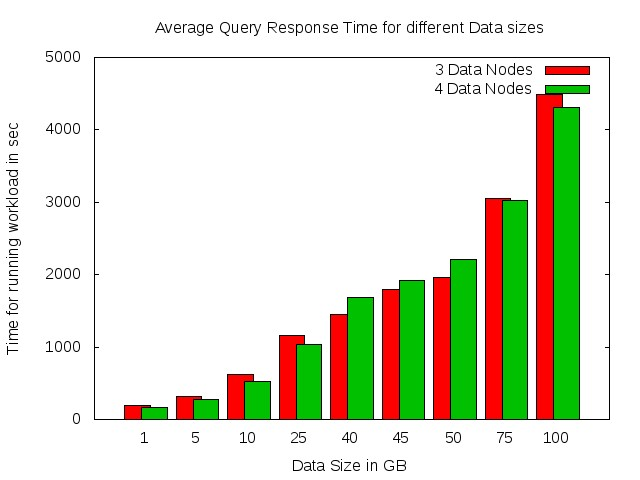
\includegraphics[width=7cm]{bar_comparison.jpeg}
 \label{barcomp}
 }
 \subfigure
 {
 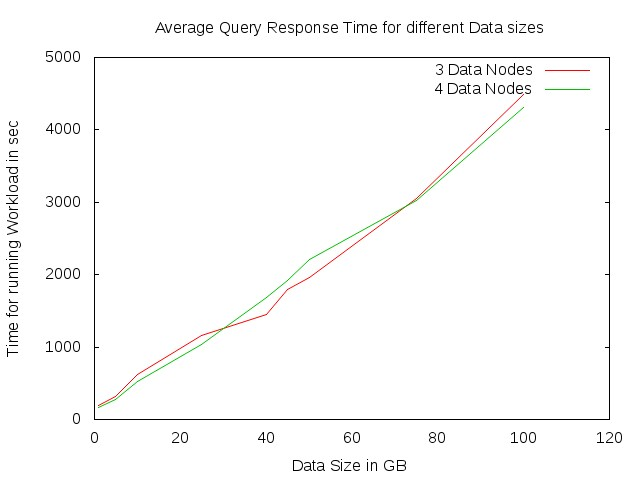
\includegraphics[width=7cm]{line_comparison.jpeg}
 \label{linecomp}
 }
\caption{Average Query Response Times for different data sizes}
\end{figure}

On observing the above graphs, we notice that intially, the average query response time using 4 datanodes was less than that using 3 datanodes.
However, gradually, as the data size increased, we see opposite behavior i.e. the average response time for 4 datanodes was more in comparison
to that for 3 datanodes. Furthermore, when the data size was increased further, the average response time behavior becomes same as it was 
initally.
\\\noindent
The average query response time is affected by a combination of multiple factors. The execution of queries on HDFS system involves division
and distribution of work across multiple nodes. The intermediate results are transferred across the system, combined and compiled to produce
the final result. Initially, when the data size is small, the intermediate results produced are also small in size. So the time consumed for 
transfer over the network is not a significant factor. However, with increase in data size, the size of the intermediate results is also found 
to be large. Also, it is observed that intensive amount of swapping takes place at each node. Thus, the time consumed for transfer over a larger 
network and that utilized in swapping dominates over faster computation due to distribution of workload across more number of nodes. This 
results in the change of behavior as observed in the graph. On further increasing the data size, we observe that the effect of intensive
swapping becomes constant when the swap space is utilized to its maximum limit. Hence, distribution of workload across more nodes becomes the 
dominating factor in comparison to the network transfer time because the intermediate results produced are large in size and have similar 
effect even if the network size is increased. As a result, computations are faster and the behavior of average response time becomes same as 
it was earlier.          
\newline\noindent
\newline\noindent

The  following table lists the scale factor for change in query response time with respect to that of 1 GB data:
\captionof{table}{Scale Factor for change in query response time for 3 and 4 Data nodes}
\begin{center}
\begin{tabular}{|c|c|c|}\hline
\multirow{2}{*}{Data Size} & \multicolumn{2}{c|}{Scale Factor (w.r.t 1GB)}\\
\cline{2-3}
& 3 DataNodes & 4 DataNodes\\\hline
1 & 1 & 1\\
5 &  1.59 & 1.68\\
10 & 3.08 & 3.28\\
25 & 6.04 & 6.13\\
40 & 9.78 & 7.71\\
45 & 11.18 & 9.53\\
50 & 12.82 & 10.40\\
75 & 17.61 & 16.24\\
100 & 25.06 & 23.88\\\hline
\end{tabular}
\end{center}

The figures \ref{sf3} and \ref{sf4} indicate the above parameter for 3 datanodes and 4 datanodes respectively.
\begin{figure}[h]
 \centering
 \subfigure
 {
 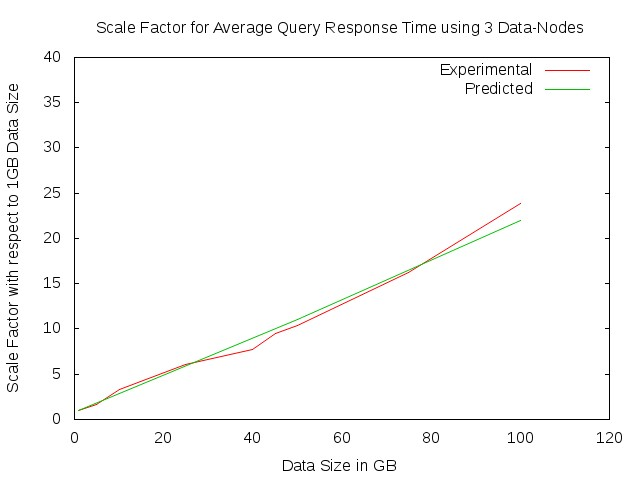
\includegraphics[width=7cm]{sf3.jpeg}
 \label{sf3}
 }
 \subfigure
 {
 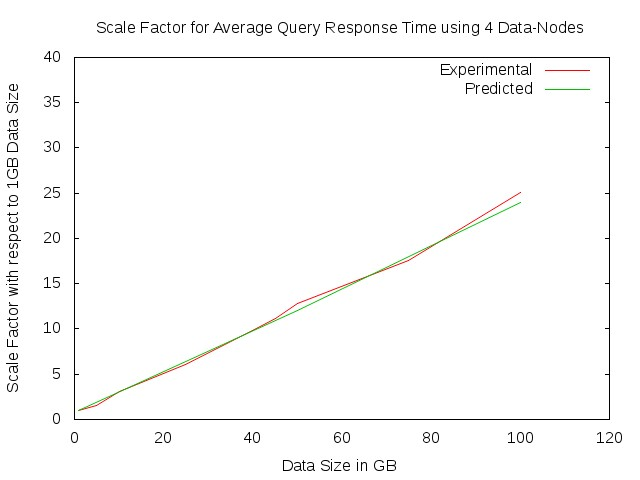
\includegraphics[width=7cm]{sf4.jpeg}
  \label{sf4}
 }
 \caption{Scale Factor for change in query response time w.r.t. 1 GB data}
\end{figure}

As shown in the graph above, we have drawn a mean line which can be extrapolated to predict the scale factors for larger data sizes.
The predicted response times thus obtained for the data sizes used in the experiment and their relative errors have been listed
in the tables below. \\\noindent
Table \ref{3tab} is for 3 datanodes while table \ref{4tab} is for 4 datanodes.\\
\captionof{table}{Error in Predicted time w.r.t Experimental time for 3 Datanodes}
\begin{center}
\label{3tab}
\begin{tabular}{|c|c|c|c|}\hline
Data Size & Experimental Time (sec) & Predicted Time (sec) & Deviation (sec) \\\hline
1 & 188 & 188 & 0\\
5 & 317 & 338 & 21\\
10 & 617 & 526 & 91\\
25 & 1154 & 1090 & 64\\
40 & 1451 & 1654 & 103\\
45 & 1793 & 1842 & 49\\
50 & 1956 & 2030 & 74\\
75 & 3054 & 2970 & 84\\
100 & 4491 & 3910 & 481\\\hline
\multicolumn{3}{|c|}{Mean Deviation} & 107\\\hline
\end{tabular}
\end{center}

\captionof{table}{Error in Predicted time w.r.t Experimental time for 4 Data nodes}
\begin{center}
\label{4tab}
\begin{tabular}{|c|c|c|c|}\hline
Data Size & Experimental Time (sec) & Predicted Time (sec) & Deviation (sec) \\\hline
1 & 172 & 170 & 2\\
5 & 275 & 321 & 46\\
10 & 530 & 510 & 20\\
25 & 1040 & 1078 & 38\\
40 & 1682 & 1646 & 32\\
45 & 1924 & 1835 & 79\\
50 & 2205 & 2024 & 181\\
75 & 3029 & 2970 & 59\\
100 & 4312 & 3916 & 396\\\hline
\multicolumn{3}{|c|}{Mean Deviation} & 94\\\hline
\end{tabular}
\end{center}
\noindent
As noted from the above table, graphical analysis can be used to predict the average query response time with acceptable devaition
upto a certain extent.

%%%%%%%%%%%%%%%%%%%%%%%%%%%%%%%%%%%%%%%%%%%%%%%%%%%%%%%%%%%%%%%%%%%%%%%%%%%%%%%%%%%%%%%%%%%%%%%%%%%%%%%%%%%%%%%%%%%%%%%%%%%%%%%%%%%%%%%%%%%%%%
%%%%%%%%%%%%%%%%%%%%%%%%%%%%%%%%%%%%%%%%%%%%%%%%%%%%%%%%  Conclusion  and Future Work  %%%%%%%%%%%%%%%%%%%%%%%%%%%%%%%%%%%%%%%%%%%%%%%%%%%%%%%
%%%%%%%%%%%%%%%%%%%%%%%%%%%%%%%%%%%%%%%%%%%%%%%%%%%%%%%%%%%%%%%%%%%%%%%%%%%%%%%%%%%%%%%%%%%%%%%%%%%%%%%%%%%%%%%%%%%%%%%%%%%%%%%%%%%%%%%%%%%%%%

\chapter{Conclusion and Future Work}
In this experiment, we have designed a specific workload for benchmarking a HDFS system built using commodity machines. 
We have also presented the rationale behind the pattern of system response time observed during the experiment as we changed the size of 
the cluster. Based on the experimental results obtained, we have used graphical analysis to predict the expected response time for larger 
data sets. 
% As an illustration, we have presented the graphs generated by Ganglia depicting some of the performance metrics of the HDFS 
% cluster during a particular run of the experiment.
\\\noindent
\newline\noindent
In future, we plan to expand the size of the cluster furthermore and work on developing a graphical analysis to predict the optimum size of 
cluster required to work with data of a particular size. Also, we intend to make an open source release of the customized benchmarking suite 
used in the experiment available to the Big Data community.
\bibliographystyle{ieeetr}
\bibliography{biblio}

\chapter*{Appendix A}
\label{appendixa}
This appendix lists the 9 queries in english and sql-mr.
\begin{itemize}
 \item \textbf{Query 1}. Find the last 5 products that are mostly viewed before a given product was purchased online. Only products in 
 certain categories and viewed within 10 days before the purchase date are considered.
\lstset{language=SQL,basicstyle=\ttfamily}
\begin{lstlisting}[frame=single]
SELECT lastviewed_item , purchased_item , COUNT (*)
FROM nPath ( ON web_clickstreams
PARTITION BY wcs_user_sk
ORDER BY wcs_click_date_sk,wcs_click_time_sk
MODE (’NONOVERLAPPING’)
PATTERN ( ’A +.B’)
SYMBOLS ( true AS A , wcs_sales_sk IS NOT NULL AS B )
RESULT (
LAST ( wcs_item_sk OF A ) AS lastviewed_item ,
LAST ( wcs_click_date_sk OF A ) AS lastviewed_date ,
FIRST ( wcs_item_sk OF B ) AS purchased_item ,
FIRST ( wcs_click_date_sk OF B) AS purchased_date
)
)
WHERE purchased_item = 16891
AND purchased_date - lastviewed_date < 11
GROUP BY 1 ,2;
\end{lstlisting}
\item \textbf{Query 2}. For online sales, compare the total sales in which customers checked online reviews before making the purchase and 
that of sales in which customers did not read reviews. Consider only online sales for a specific category in a given year.
\begin{lstlisting}[frame=single]
BEGIN ;
DROP VIEW clicks ;
CREATE VIEW clicks AS (
SELECT c.wcs_item_sk AS item ,
c.wcs_user_sk AS uid ,
c.wcs_click_date_sk AS c_date ,
c.wcs_click_time_sk AS c_time ,
c.wcs_sales_sk AS sales_sk ,
w.wp_type AS wpt
FROM web_clickstreams c , web_page w
WHERE c.wcs_web_page_sk = w.wp_web_page_sk
and c.wcs_user_sk IS NOT NULL
);
DROP VIEW sales_review;
CREATE VIEW sales_review AS (
SELECT s_sk
FROM nPath ( ON clicks
PARTITION BY uid
ORDER BY c_date , c_time
MODE (’NONOVERLAPPING’)
PATTERN ( ’A +. C *. B ’)
SYMBOLS ( wpt = ’ review ’ AS A , TRUE AS C ,
sales_sk IS NOT NULL AS B )
RESULT ( FIRST ( c_date OF B ) AS s_date ,
FIRST ( sales_sk OF B ) AS s_sk ) )
WHERE s_date > 2451424 AND s_date <2451424+365
);
SELECT SUM ( CASE WHEN ws.ws_sk IN 
( SELECT * FROM sales_review)
THEN ws_net_paid
ELSE 0 END ) AS review_sales_amount ,
SUM ( ws_net_paid) -
SUM ( CASE WHEN ws.ws_sk IN 
( SELECT * FROM sales_review)
THEN ws_net_paid
ELSE 0 END ) AS no_review_sales_amount
FROM web_sales ws
WHERE ws.ws_sold_date_sk > 2451424
AND ws.w s_sold_date_sk <2451424+365;
END ;
\end{lstlisting}

\item \textbf{Query 3}. (TPC-DS 48) Calculate the total sales by different types of customers (e.g., based on marital status, education status),
sales price and different combinations of state and sales profit.
\begin{lstlisting}[frame=single]
SELECT SUM ( ss_quantity)
FROM store_sales , store , customer_demographics ,
customer_address , date_dim
WHERE s_store_sk =ss_store_sk
AND ss_sold_date_sk = d_date_sk
AND d_year = 1998
AND (( cd_demo_sk = ss_cdemo_sk
AND cd_marital_status = ’M ’
AND cd_education_status = ’4 yr Degree ’
AND ss_sales_price between 100.00 AND 150.00)
OR
( cd_demo_sk = ss_cdemo_sk
AND cd_marital_status = ’M ’
AND cd_education_status = ’4 yr Degree ’
AND ss_sales_price between 50.00 AND 100.00)
OR
( cd_demo_sk = ss_cdemo_sk
AND cd_marital_status = ’M ’
AND cd_education_status = ’4 yr Degree ’
AND ss_sales_price between 150.00 AND 200.00) )
AND ((ss_addr_sk = ca_address_sk
AND ca_country = ’ United States ’
AND ca_state in (’KY’,’GA’,’NM’)
AND ss_net_profit between 0 AND 2000)
OR
( ss_addr_sk = ca_address_sk
AND ca_country = ’United States’
AND ca_state in (’MT’,’OR’,’IN’)
AND ss_net_profit between 150 AND 3000)
OR
( ss_addr_sk = ca_address_sk
AND ca_country = ’United States’
AND ca_state in (’WI’,’MO’,’WV’)
AND ss_net_profit between 50 AND 25000) ) ;
\end{lstlisting}

\item \textbf{Query 4}. For all products, extract sentences from its product reviews that contain positive or negative sentiment and 
display the sentiment polarity of the extracted sentences.
\begin{lstlisting}[frame=single]
SELECT pr_item_sk , out_content , 
out_polarity , out_sentiment_words
FROM ExtractSentiment
( ON product_reviews100
TEXT_COLUMN (’pr_review_content’)
MODEL (’dictionary’)
LEVEL (’ sentence ’)
ACCUMULATE (’pr_item_sk’)
)
WHERE out_polarity = ’NEG’
OR out_polarity = ’POS’;
\end{lstlisting}

\item \textbf{Query 5}. For a given product, measure the correlation of sentiments, including the number of reviews and average review 
ratings, on product monthly revenues.
\begin{lstlisting}[frame=single]
BEGIN ;
DROP VIEW IF EXISTS review_stats;
CREATE VIEW review_stats AS (
SELECT p.pr_item_sk AS pid ,
CAST ( p.r_count AS INT ) AS reviews_count ,
CAST ( p.avg_rating AS INT ) AS avg_rating ,
CAST ( s.revenue AS INT ) AS m_revenue
FROM ( SELECT pr_item_sk , COUNT (*) AS r_count ,
AVG ( pr_review_rating) AS avg_rating
FROM product_reviews
WHERE pr_item_sk IS NOT NULL
GROUP BY 1) p
JOIN
( SELECT ws_item_sk , SUM (ws_net_paid) AS revenue
FROM web_sales
WHERE ws_sold_date_sk > 2452642 -30
AND ws_sold_date_sk < 2452642
AND ws_item_sk IS NOT NULL
GROUP BY 1) s
ON p.pr_item_sk=s.ws_item_sk) ;
SELECT *
FROM corr_reduce ( ON
corr_map ( ON
review_stats
COLUMNS ( ’[ m_revenue:reviews_count] ,[ m_revenue:avg_rating] ’)
KEY_NAME ( ’k ’)
)
PARTITION BY k) ;
DROP VIEW review_stats;
END ; 
\end{lstlisting}

\item \textbf{Query 6}. (TPC-DS 90) What is the ratio between the number of items sold over the internet in the morning (8 to 9am) to the 
number of items sold in the evening (7 to 8pm) of customers with a specified number of dependents. Consider only websites with a high amount 
of content.
\begin{lstlisting}[frame=single]
SELECT CAST (amc AS DECIMAL (15 ,4)) / CAST ( pmc AS DECIMAL (15,4)) am_pm_ratio
FROM ( SELECT COUNT (*) amc
FROM web_sales,household_demographics , time_dim , web_page wp
WHERE ws_sold_time_sk = time_dim.t_time_sk
AND ws_ship_hdemo_sk = household_demographics.hd_demo_sk
AND ws_web_page_sk = wp.wp_web_page_sk
AND time_dim.t_hour BETWEEN 8 AND 8+1
AND household_demographics.hd_dep_count = 5
AND wp . w p _ c h a r _ c o u n t BETWEEN 5000 AND 5200) at ,
( SELECT COUNT (*) pmc
FROM web_sales , h o u s e h o l d _ d e m o g r a p h i c s , time_dim , web_page wp
WHERE w s _ s o l d _ t i m e _ s k = time_dim . t _ t i m e _ s k
AND w s _ s h i p _ h d e m o _ s k = h o u s e h o l d _ d e m o g r a p h i c s. h d _ d e m o _ s k
AND w s _ w e b _ p a g e _ s k = wp . w p _ w e b _ p a g e _ s k
AND time_dim . t_hour BETWEEN 19 AND 19+1
AND h o u s e h o l d _ d e m o g r a p h i c s. h d _ d e p _ c o u n t = 5
AND wp . w p _ c h a r _ c o u n t BETWEEN 5000 AND 5200) pt
ORDER BY a m _ p m _ r a t i o ;
\end{lstlisting}

\item \textbf{Query 7}. (TPC-DS 61) Find the ratio of items sold with and without promotions in a given month and year. Only items in certain 
categories sold to customers living in a specific time zone are considered.
\begin{lstlisting}[frame=single]
SELECT promotions , total ,
CAST ( p r o m o t i o n s AS DECIMAL (15 ,4) ) /
CAST ( total AS DECIMAL (15 ,4) ) * 100
FROM ( SELECT SUM ( s s _ e x t _ s a l e s _ p r i c e) p r o m o t i o n s
FROM store_sales , store , promotion , date_dim ,
customer , customer_address , item
WHERE s s _ s o l d _ d a t e _ s k = d _ d a t e _ s k
AND s s _ s t o r e _ s k = s _ s t o r e _ s k
AND s s _ p r o m o _ s k = p _ p r o m o _ s k
AND s s _ c u s t o m e r _ s k= c _ c u s t o m e r _ s k
AND c a _ a d d r e s s _ s k = c _ c u r r e n t _ a d d r _ s k
AND s s _ i t e m _ s k = i _ i t e m _ s k
AND c a _ g m t _ o f f s e t = -7
AND i _ c a t e g o r y = ’ Jewelry ’
AND ( p _ c h a n n e l _ d m a i l = ’Y ’ OR p _ c h a n n e l _ e m a i l = ’Y ’
OR p _ c h a n n e l _ t v = ’Y ’)
AND s _ g m t _ o f f s e t = -7
AND d_year = 2001
AND d_moy = 12) p r o m o t i o n a l_ sal es ,
( SELECT sum ( s s _ e x t _ s a l e s _ p r i c e) total
FROM store_sales , store , date_dim ,
customer , customer_address , item
WHERE s s _ s o l d _ d a t e _ s k = d _ d a t e _ s k
AND s s _ s t o r e _ s k = s _ s t o r e _ s k
AND s s _ c u s t o m e r _ s k= c _ c u s t o m e r _ s k
AND c a _ a d d r e s s _ s k = c _ c u r r e n t _ a d d r _ s k
AND s s _ i t e m _ s k = i _ i t e m _ s k
AND c a _ g m t _ o f f s e t = -7
AND i _ c a t e g o r y = ’ Jewelry ’
AND s _ g m t _ o f f s e t = -7
AND d_year = 2001
AND d_moy = 12) a l l _ s a l e s
ORDER BY promotions , total ;
\end{lstlisting}

\item \textbf{Query 8}. For a given product, measure the effect of competitors’ prices on products’ in-store and online sales. 
(Compute the cross-price elasticity of demand for a given product).
\begin{lstlisting}[frame=single]
BEGIN ;
CREATE VIEW c o m p e t i t o r _ p r i c e _ v i e w AS
( SELECT i_item_sk , ( i m p _ c o m p e t i t o r _ p r i c e - i _ c u r r e n t _ p r i c e)
/ i _ c u r r e n t _ p r i c e AS price_change , imp_start_date ,
i m p _ e n d _ d a t e - i m p _ s t a r t _ d a t e AS no_days
FROM item , i t e m _ m a r k e t p r i c e s
WHERE i m p _ i t e m _ s k = i _ i t e m _ s k
AND i _ i t e m _ s k in (7 ,17)
AND i m p _ c o m p e t i t o r _ p r i c e < i _ c u r r e n t _ p r i c e) ;
CREATE VIEW s e l f _ w s _ v i e w AS
( SELECT ws_item_sk ,
SUM ( CASE WHEN w s _ s o l d _ d a t e _ s k >= c . i m p _ s t a r t _ d a t e
AND w s _ s o l d _ d a t e _ s k < c . i m p _ s t a r t _ d a t e + c . no_days
THEN w s _ q u a n t i t y ELSE 0 END ) AS current_ws ,
SUM ( CASE WHEN w s _ s o l d _ d a t e _ s k >= c . i m p _ s t a r t _ d a t e - c . no_days
AND w s _ s o l d _ d a t e _ s k < c . i m p _ s t a r t _ d a t e
THEN w s _ q u a n t i t y ELSE 0 END ) AS prev_ws
FROM web_sales , c o m p e t i t o r _ p r i c e _ v i e w c
WHERE w s _ i t e m _ s k = c . i _ i t e m _ s k
GROUP BY 1) ;
CREATE VIEW s e l f _ s s _ v i e w
( SELECT ss_item_sk ,
SUM ( CASE WHEN
AND
THEN
SUM ( CASE WHEN
AND
AS
s s _ s o l d _ d a t e _ s k >= c . i m p _ s t a r t _ d a t e
s s _ s o l d _ d a t e _ s k < c . i m p _ s t a r t _ d a t e + c . no_days
s s _ q u a n t i t y ELSE 0 END ) AS current_ss ,
s s _ s o l d _ d a t e _ s k >= c . i m p _ s t a r t _ d a t e - c . no_days
ss_sold_date_sk < c. imp_start_date190
THEN s s _ q u a n t i t y ELSE 0 END ) AS prev_ss
FROM store_sales , c o m p e t i t o r _ p r i c e _ v i e w c
WHERE c . i _ i t e m _ s k = s s _ i t e m _ s k
GROUP BY 1) ;
SELECT i_item_sk , ( c u r r e n t _ s s + current_ws - prev_ss - prev_ws )
/ (( prev_ss + prev_ws ) * p r i c e _ c h a n g e) AS c r o s s _ p r i c e _ e l a s t i c i t y
FROM c o m p e t i t o r _ p r ic e_ vi ew , self_ws_view , s e l f _ s s _ v i e w
WHERE i _ i t e m _ s k = w s _ i t e m _ s k
AND i _ i t e m _ s k = s s _ i t e m _ s k;
DROP VIEW s e l f _ w s _ v i e w;
DROP VIEW s e l f _ s s _ v i e w;
DROP VIEW c o m p e t i t o r _ p r i c e _ v i e w;
END ;
\end{lstlisting}

\item \textbf{Query 9}.Perform category affinity analysis for products purchased online together.
\begin{lstlisting}[frame=single]
CREATE VIEW c_affinity_input AS
( SELECT i.i_category_id AS category_cd ,
s.ws_bill_customer_sk AS customer_id
FROM web_saless INNER JOIN item i
ON s.ws_item_sk=i_item_sk
WHERE i.i_category_id IS NOT NULL);
SELECT *
FROM cfilter ( ON
( SELECT 1)
PARTITION BY 1
DATABASE (’benchmark’)
USERID (’benchmark’)
PASSWORD (’benchmark’)
INPUTTABLE (’benchmark.c_affinity_input’)
OUTPUTTABLE (’c_affinity_out’)
DROPTABLE (’true’)
INPUTCOLUMNS (’category_cd’)
JOINCOLUMNS (’customer_id’));
SELECT * FROM c_affinity_out;
DROP TABLE IF EXISTS c_affinity_out;
DROP VIEW IF EXISTS c_affinity_input;
\end{lstlisting}
\end{itemize}


\end{document}